%  sample eprint article in LaTeX           --- M. Peskin, 9/7/00
%  modified for LHCP2017, lhcp2017@sjtu.edu.cn
%  This file is part of a tar file, which can be downloaded from the LHCP2017 indico site. 
%   https://indico.cern.ch/event/517784/overview 
% 


\documentclass[10pt]{article}
\usepackage{graphicx}



%%%%%%%%%%%%%%%%%%%%%%%%%%%%%%%%%%%%%%%%%%%%%%%%%%%%%%%%%%%%%%%%%%%%%%%%%%%%
%   document style macros
%%%%%%%%%%%%%%%%%%%%%%%%%%%%%%%%%%%%%%%%%%%%%%%%%%%%%%%%%%%%%%%%%%%%%%%%%%%%
\def\Title#1{\begin{center} {\Large #1 } \end{center}}
\def\Author#1{\begin{center}{ \sc #1} \end{center}}
\def\Address#1{\begin{center}{ \it #1} \end{center}}
\def\andauth{\begin{center}{and} \end{center}}
\def\submit#1{\begin{center}Submitted to {\sl #1} \end{center}}
\newcommand\pubblock{\rightline{\begin{tabular}{l} Proceedings of the Fifth Annual LHCP\\ \pubnumber\\
         \pubdate  \end{tabular}}}

\newenvironment{Abstract}{\begin{quotation} \begin{center} 
             \large ABSTRACT \end{center}\bigskip 
      \begin{center}\begin{large}}{\end{large}\end{center} \end{quotation}}

\newenvironment{Presented}{\begin{quotation} \begin{center} 
             PRESENTED AT\end{center}\bigskip 
      \begin{center}\begin{large}}{\end{large}\end{center} \end{quotation}}

\def\Acknowledgements{\bigskip  \bigskip \begin{center} \begin{large}
             \bf ACKNOWLEDGEMENTS \end{large}\end{center}}
%%%%%%%%%%%%%%%%%%%%%%%%%%%%%%%%%%%%%%%%%%%%%%%%%%%%%%%%%%%%%%%%%%%%%%%%%%%%
%  personal abbreviations and macros
%    the following package contains macros used in this document:
\input econfmacros.tex
%%%%%%%%%%%%%%%%%%%%%%%%%%%%%%%%%%%%%%%%%%%%%%%%%%%%%%%%%%%%%%%%%%%%%%%%%%%

\textwidth=6.5in  \textheight=8.75in
\hoffset=-.85in
\voffset=-0.6in

%%  DO NOT CHANGE anything above.

% include packages you will need
\usepackage{color}


%%%%%%%%%%%%%%%%%%%%%%%%%%%%%%%%%%%%%%%%%%%%%%%%%%%%%%%%%%%%%%%%%%%%
% basic data for the eprint:
%%%%%%%%%%%%%%%%%%%%%%%%%%%%%%%%%%%%%%%%%%%%%%%%%%%%%%%%%%%%%%%%%%%%

% Instruction:
% Please change each of the following fields:
%

%% preprint number data:
% If there is a preprint number from your institute, or experiment note number, please fill it in 
\newcommand\pubnumber{CMS-CR-2017/XXX}
% \newcommand\pubnumber{ }

%% date
\newcommand\pubdate{\today}

%%  Affiliation
\def\affiliation{
On behalf of the ATLAS and CMS Collaborations, \\
Instituto de F\'isica de Cantabria \\
(CSIC - Universidad de Cantabria), Spain}

%% Acknowledge the support
%%% \def\support{\footnote{Work supported by XYZ Foundation.}}



\begin{document}

% large size for the first page
\large
\begin{titlepage}
\pubblock


%% Change the title, name, abstract
%% Title 
\vfill
\Title{New results on Higgs properties}
\vfill

%  if you need to add the support use this, fill the \support definition above. 
%   \Author{ FIRSTNAME LASTNAME \support }
\Author{J\'onatan Piedra}
\Address{\affiliation}
\vfill
\begin{Abstract}
We present the latest ATLAS and CMS measurements of several Higgs properties,
such as signal-strength modifiers for the main production modes, fiducial and
differential cross sections, and the Higgs mass. We have analyzed the 13~TeV
proton-proton LHC collision data recorded in 2016, corresponding to integrated
luminosities up to 36.1~${\rm fb}^{-1}$. Results for the
${\rm H\to ZZ}\to 4\ell$ (${\rm \ell = e\mu}$),
${\rm H}\to\gamma\gamma$, and
${\rm H}\to\tau\tau$
decay channels are presented. In addition, searches for new phenomena in the
${\rm H}\to\gamma\gamma + E_{\rm T}^{\rm miss}$ and
${\rm H}\to{\rm b\bar{b}} + E_{\rm T}^{\rm miss}$ decay channels are presented.
\end{Abstract}
\vfill

% DO NOT CHANGE 
\begin{Presented}
The Fifth Annual Conference\\
 on Large Hadron Collider Physics \\
Shanghai Jiao Tong University, Shanghai, China\\ 
May 15-20, 2017
\end{Presented}
\vfill
\end{titlepage}
\def\thefootnote{\fnsymbol{footnote}}
\setcounter{footnote}{0}
%

% normal size for the rest
\normalsize 

%% Your paper should be entered below. 


%~~~~~~~~~~~~~~~~~~~~~~~~~~~~~~~~~~~~~~~~~~~~~~~~~~~~~~~~~~~~~~~~~~~~~~~~~~~~~~~
\section{Introduction}
%~~~~~~~~~~~~~~~~~~~~~~~~~~~~~~~~~~~~~~~~~~~~~~~~~~~~~~~~~~~~~~~~~~~~~~~~~~~~~~~

The discovery of the Higgs boson was announced in 2012 by the ATLAS and CMS
collaborations~\cite{Aad:2012tfa,Chatrchyan:2012ufa} based on proton-proton
collisions collected at the CERN LHC at the centre of mass energies of 7 and
8~TeV. Since then a huge effort has been made in the determination of the
properties of this newly found particle. The dataset already collected at 13~TeV
allows inclusive Higgs boson measurements to be repeated. Furthermore, the
increased centre-of-mass energy results in much larger cross sections for events
at high partonic centre-of-mass energy. This implies improved sensitivity to a
variety of interesting physics processes, such as Higgs bosons produced at high
transverse momentum.

In this document we present the latest ATLAS and CMS measurements of several
Higgs properties in different decay channels, such as ${\rm H\to ZZ}$,
${\rm H\to\gamma\gamma}$ and ${\rm H\to\tau\tau}$. In addition, we also present
results on searches for phenomena beyond the Standard Model, in Higgs decays
to $\gamma\gamma$ or ${\rm b\bar{b}}$, with $E_{\rm T}^{\rm miss}$ in the final
state.


%~~~~~~~~~~~~~~~~~~~~~~~~~~~~~~~~~~~~~~~~~~~~~~~~~~~~~~~~~~~~~~~~~~~~~~~~~~~~~~~
\section{\boldmath ${\rm H}\to{\rm ZZ}$}
%~~~~~~~~~~~~~~~~~~~~~~~~~~~~~~~~~~~~~~~~~~~~~~~~~~~~~~~~~~~~~~~~~~~~~~~~~~~~~~~

The ${\rm H\to ZZ\to 4\ell}$ decay channel (${\rm \ell = e,\mu}$) has a large
signal-to-background ratio due to the complete reconstruction of the final state
decay products and excellent lepton momentum resolution, making it one of the
most important channels for studies of the Higgs boson's properties. Here we
present measurements of properties of the Higgs boson in this channel at 13~TeV,
for both the ATLAS and CMS collaborations~\cite{ATLAS-ZZ,CMS:2017jkd}.

See Figure~\ref{fig:figure-ZZ} and Table~\ref{tab:table1}. 

\begin{figure}[htb]
\centering
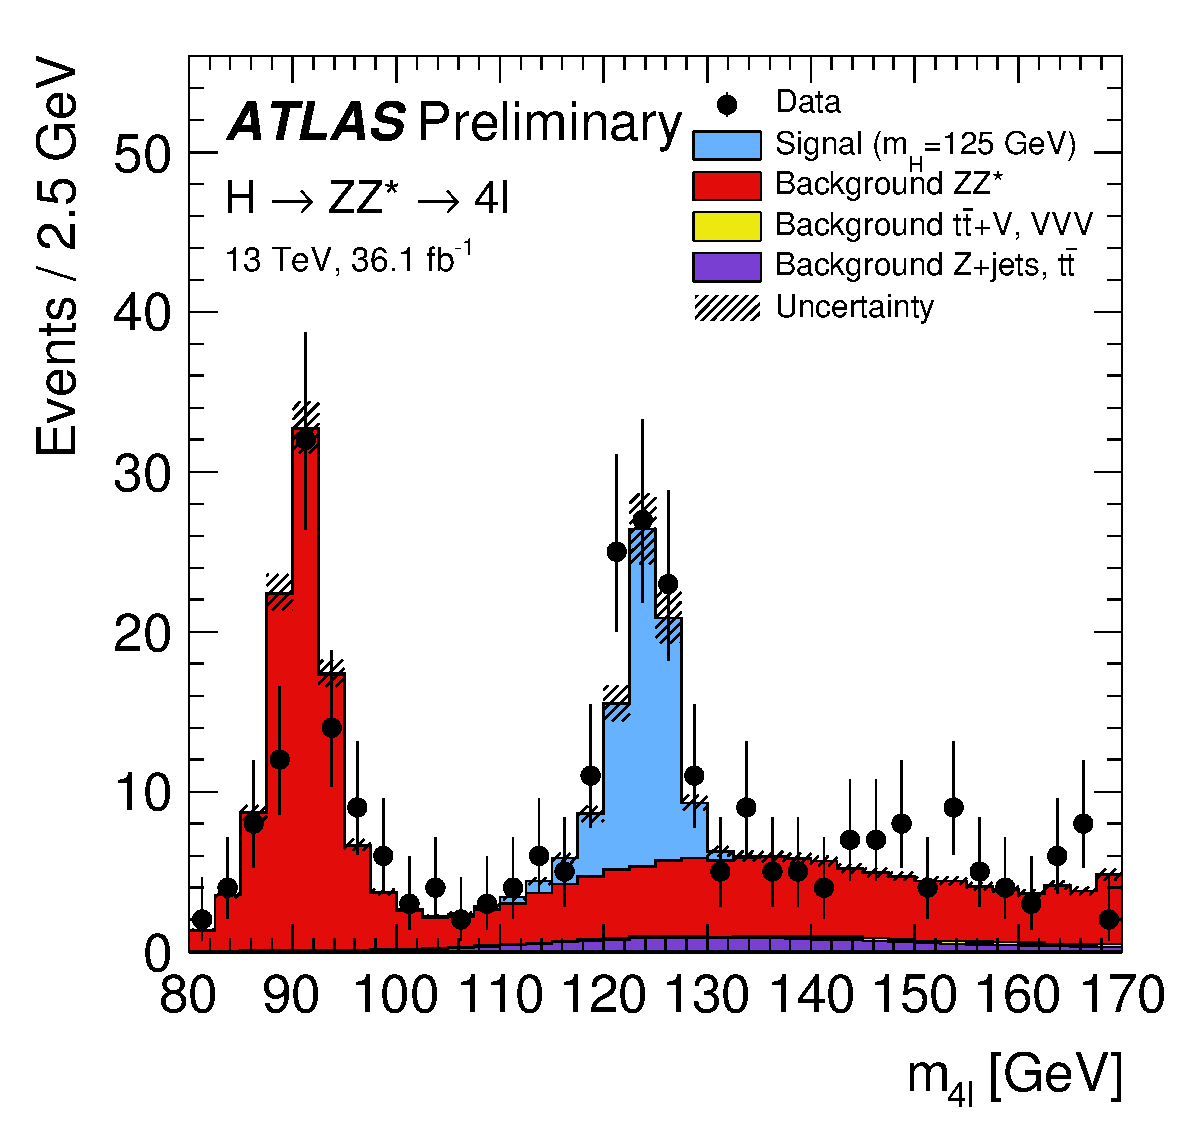
\includegraphics[height=2in]{figures/ATLAS-CONF-2017-032__fig_01__m4l.pdf}
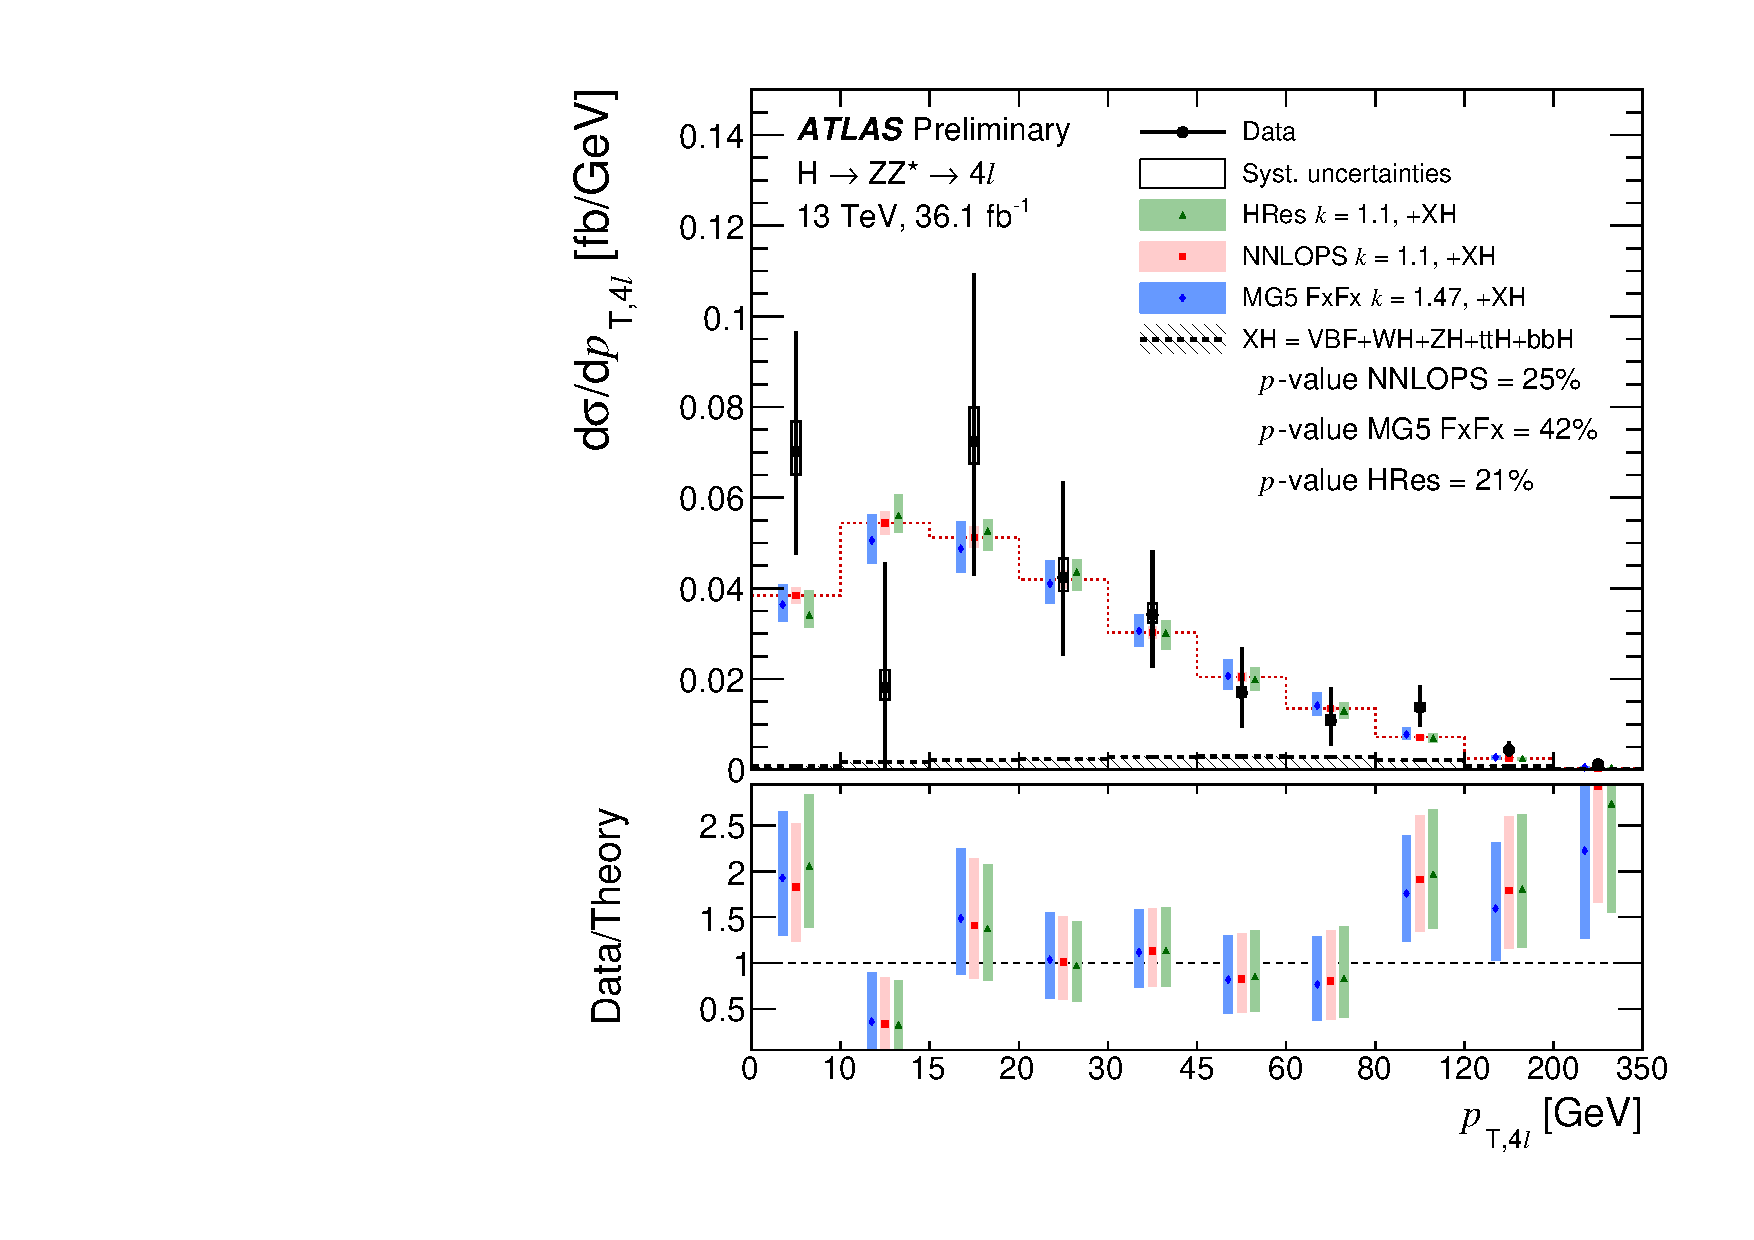
\includegraphics[height=2in]{figures/ATLAS-CONF-2017-032__fig_08a__pT4l.pdf}
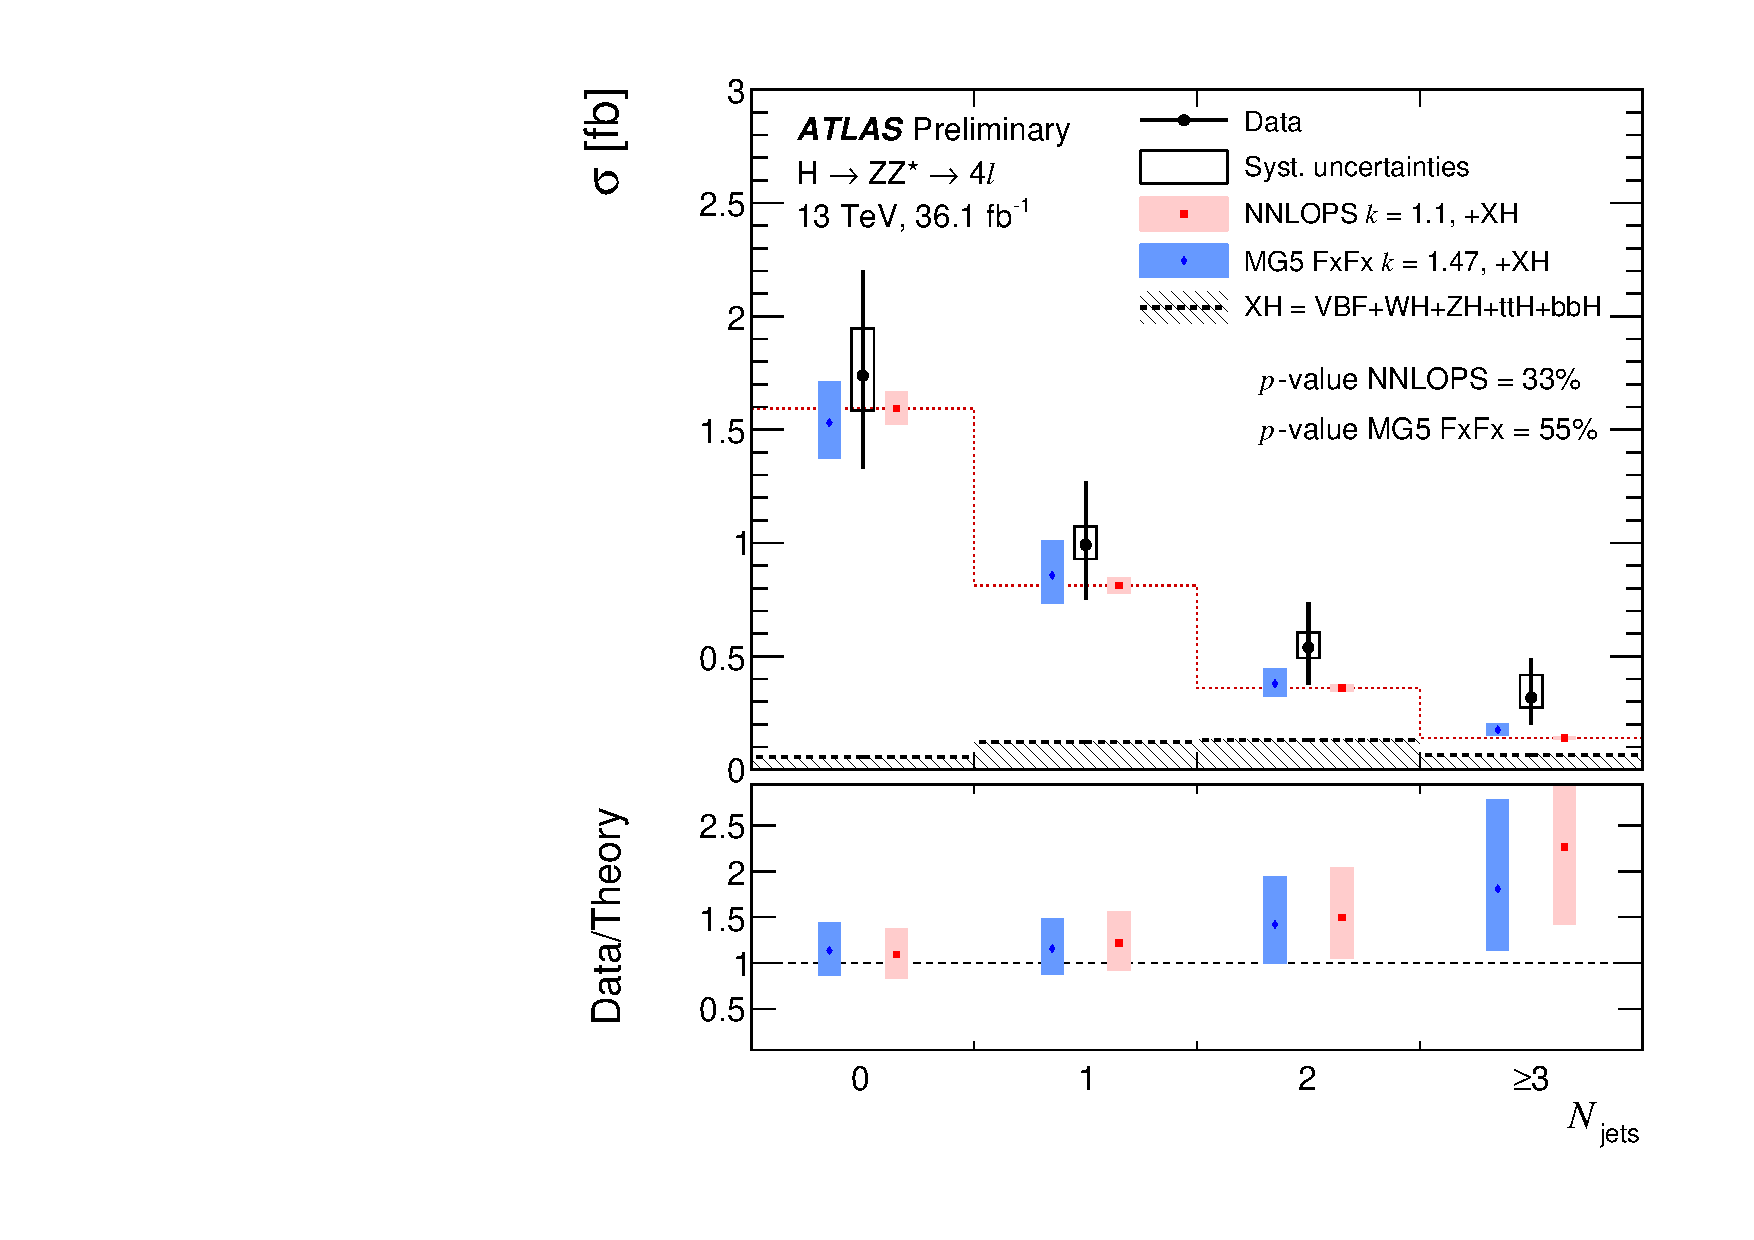
\includegraphics[height=2in]{figures/ATLAS-CONF-2017-032__fig_09a__njets.pdf}\\
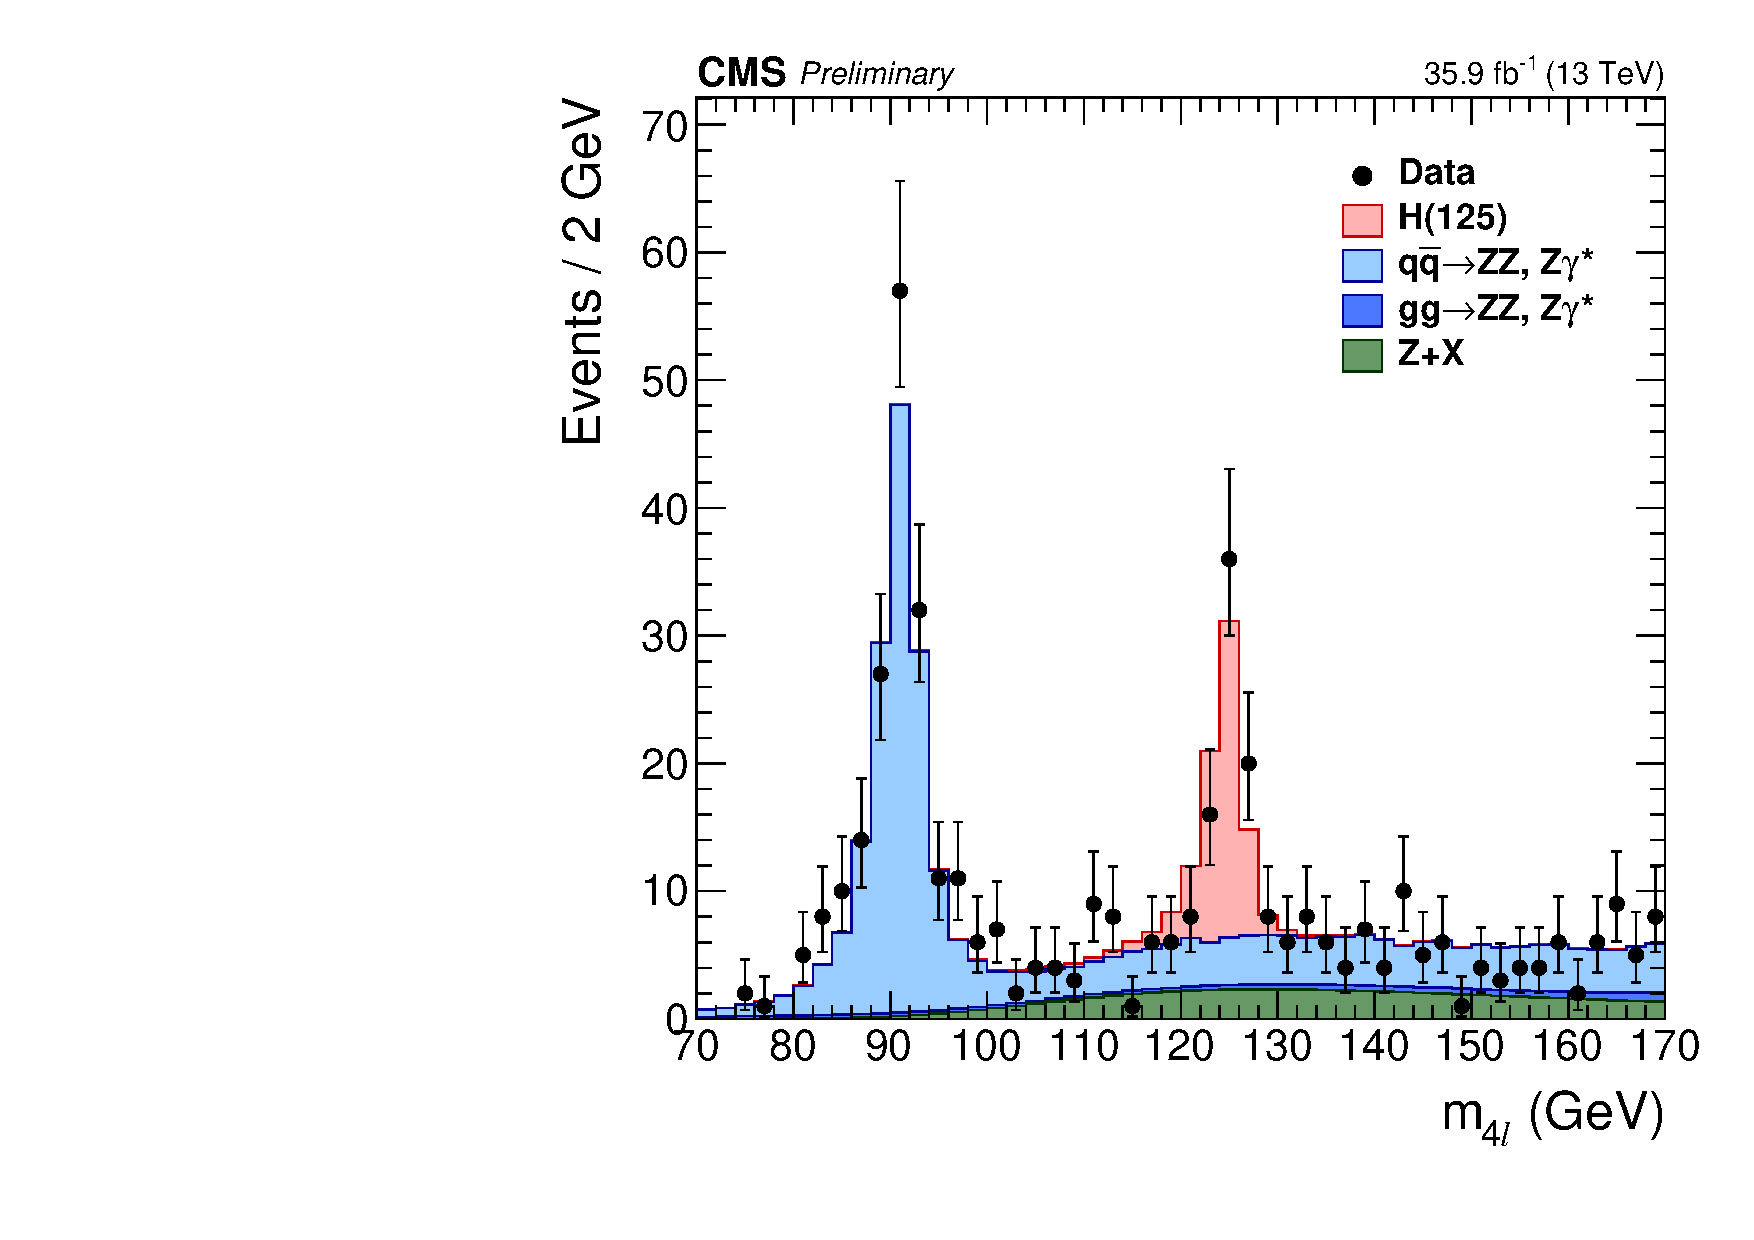
\includegraphics[height=2in]{figures/CMS-HIG-16-041__Figure_003-b__m4l.pdf}
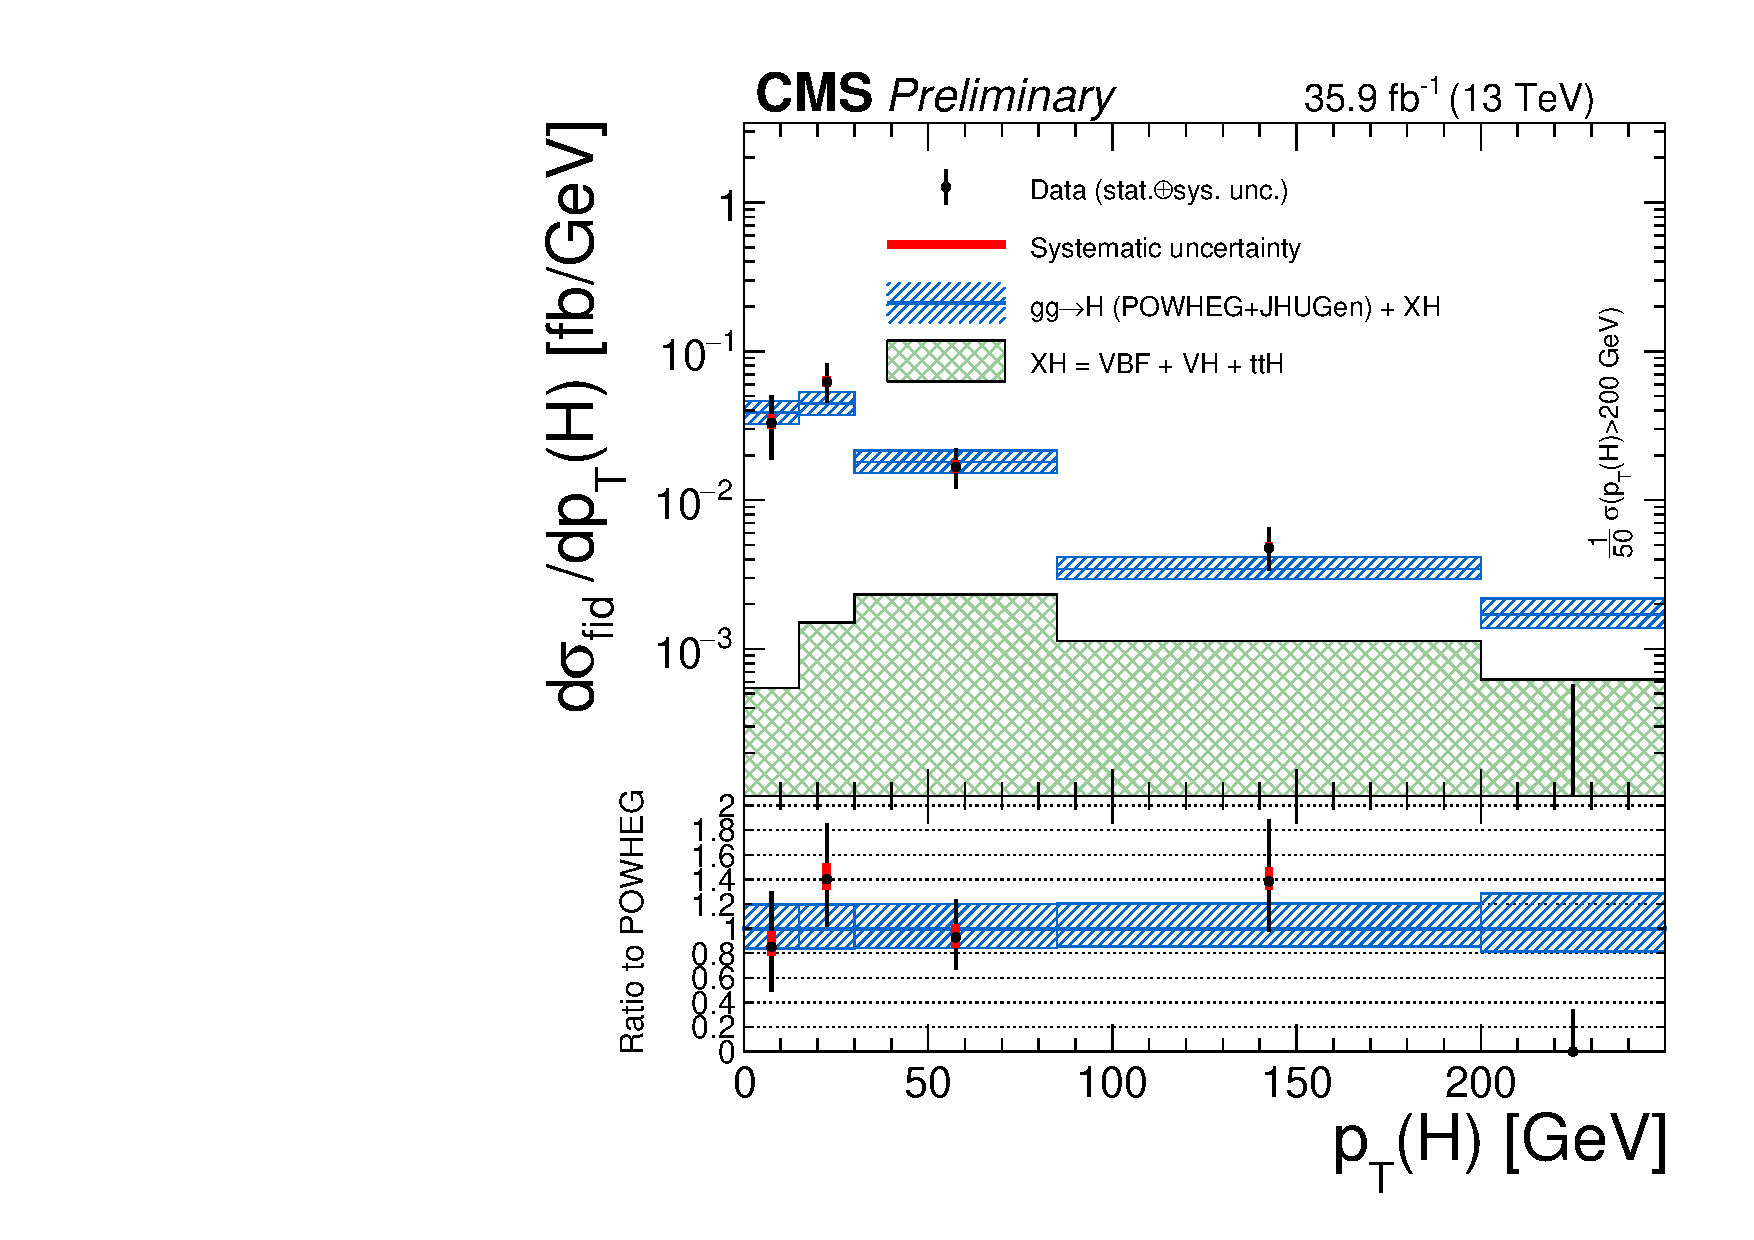
\includegraphics[height=2in]{figures/CMS-HIG-16-041__Figure_009-b__pT4l.pdf}
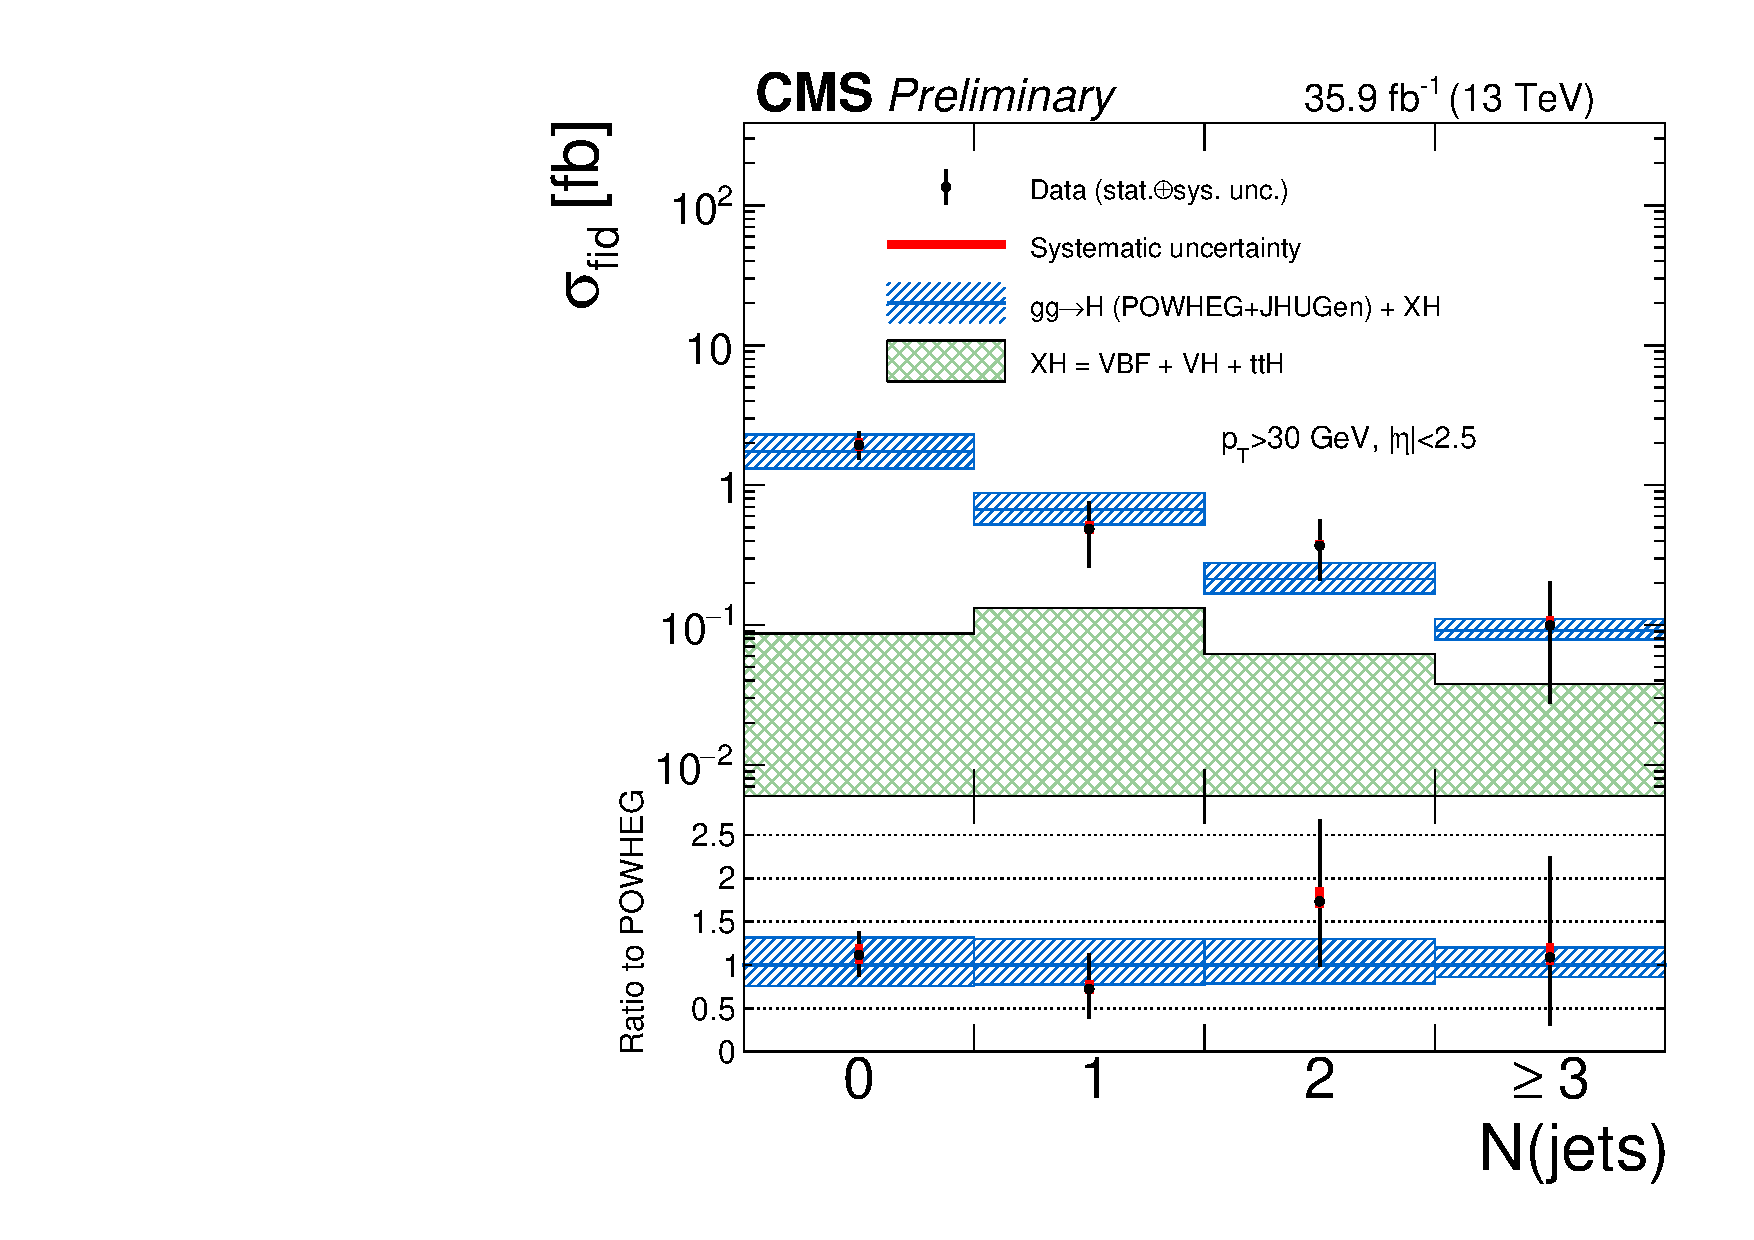
\includegraphics[height=2in]{figures/CMS-HIG-16-041__Figure_009-c__njets.pdf}
\caption{
  (Top left) ATLAS four-lepton invariant mass distribution of the selected
  events. The systematic uncertainty on the prediction is shown by the dashed
  band.
  (Top center and right) ATLAS differential fiducial cross sections, for the
  transverse momentum of the Higgs boson (center) and the number of jets (right).
  The measured cross sections are compared to different ggH predictions, and
  predictions for all other Higgs production modes XH are added.
  (Bottom left) CMS four-lepton invariant mass distribution of the selected
  events.
  (Bottom center and right) CMS differential fiducial cross sections, for the
  transverse momentum of the Higgs boson (center) and the number of jets (right).
  The sub-dominant component of the signal (VBF + VH + ttH) is denoted as XH.
}
\label{fig:figure-ZZ}
\end{figure}


\begin{table}[t]
\begin{center}
\begin{tabular}{l|ccc}  
Patient &  Initial level($\mu$g/cc) &  w. Magnet &  
w. Magnet and Sound \\ \hline
 Guglielmo B.  &   0.12     &     0.10      &     0.001  \\
 Ferrando di N. &  0.15     &     0.11      &  $< 0.0005$ \\ \hline
\end{tabular}
\caption{Place the caption here.}
\label{tab:table1}
\end{center}
\end{table}


%~~~~~~~~~~~~~~~~~~~~~~~~~~~~~~~~~~~~~~~~~~~~~~~~~~~~~~~~~~~~~~~~~~~~~~~~~~~~~~~
\section{\boldmath ${\rm H}\to\gamma\gamma$}
%~~~~~~~~~~~~~~~~~~~~~~~~~~~~~~~~~~~~~~~~~~~~~~~~~~~~~~~~~~~~~~~~~~~~~~~~~~~~~~~

See Figure~\ref{fig:figure-gg}.

\begin{figure}[htb]
\centering
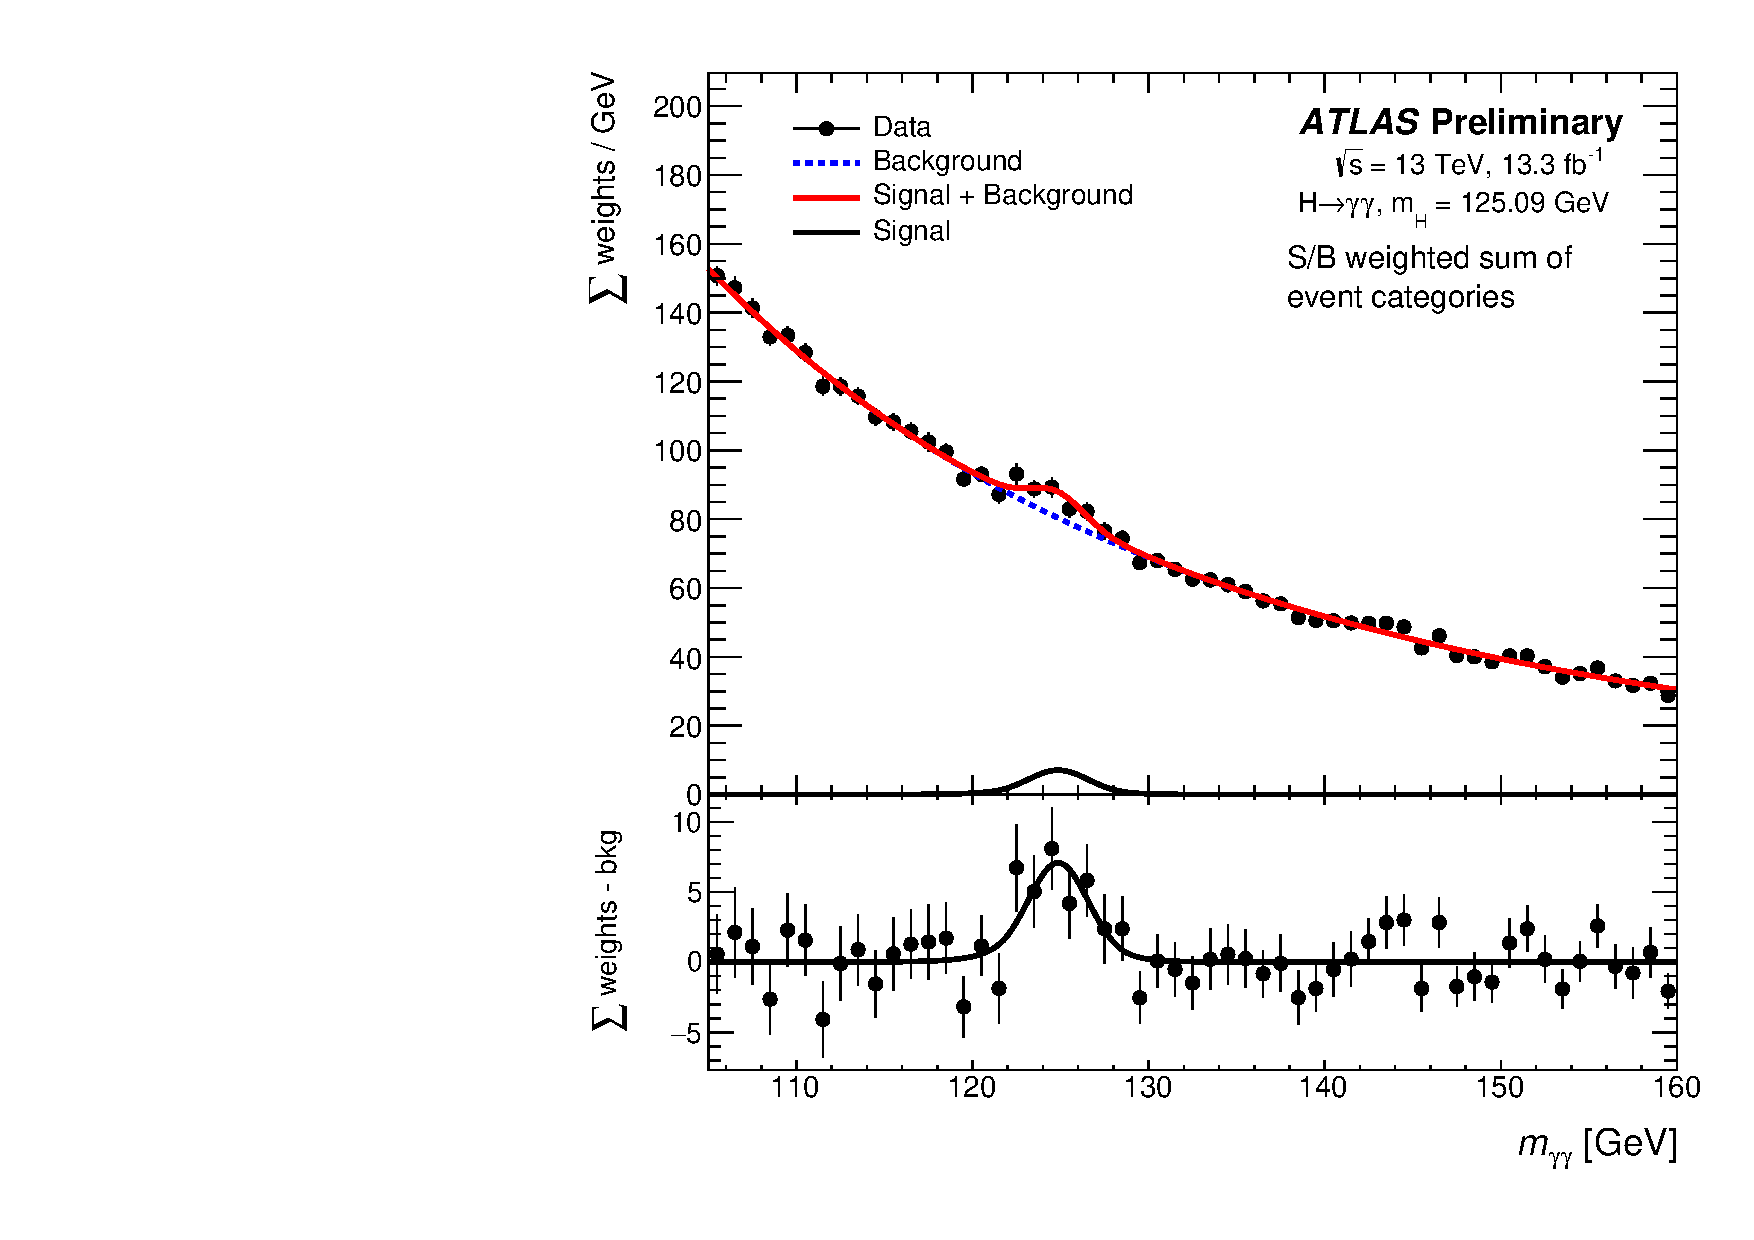
\includegraphics[height=2in]{figures/ATLAS-CONF-2016-067__fig_07__mgg.pdf}
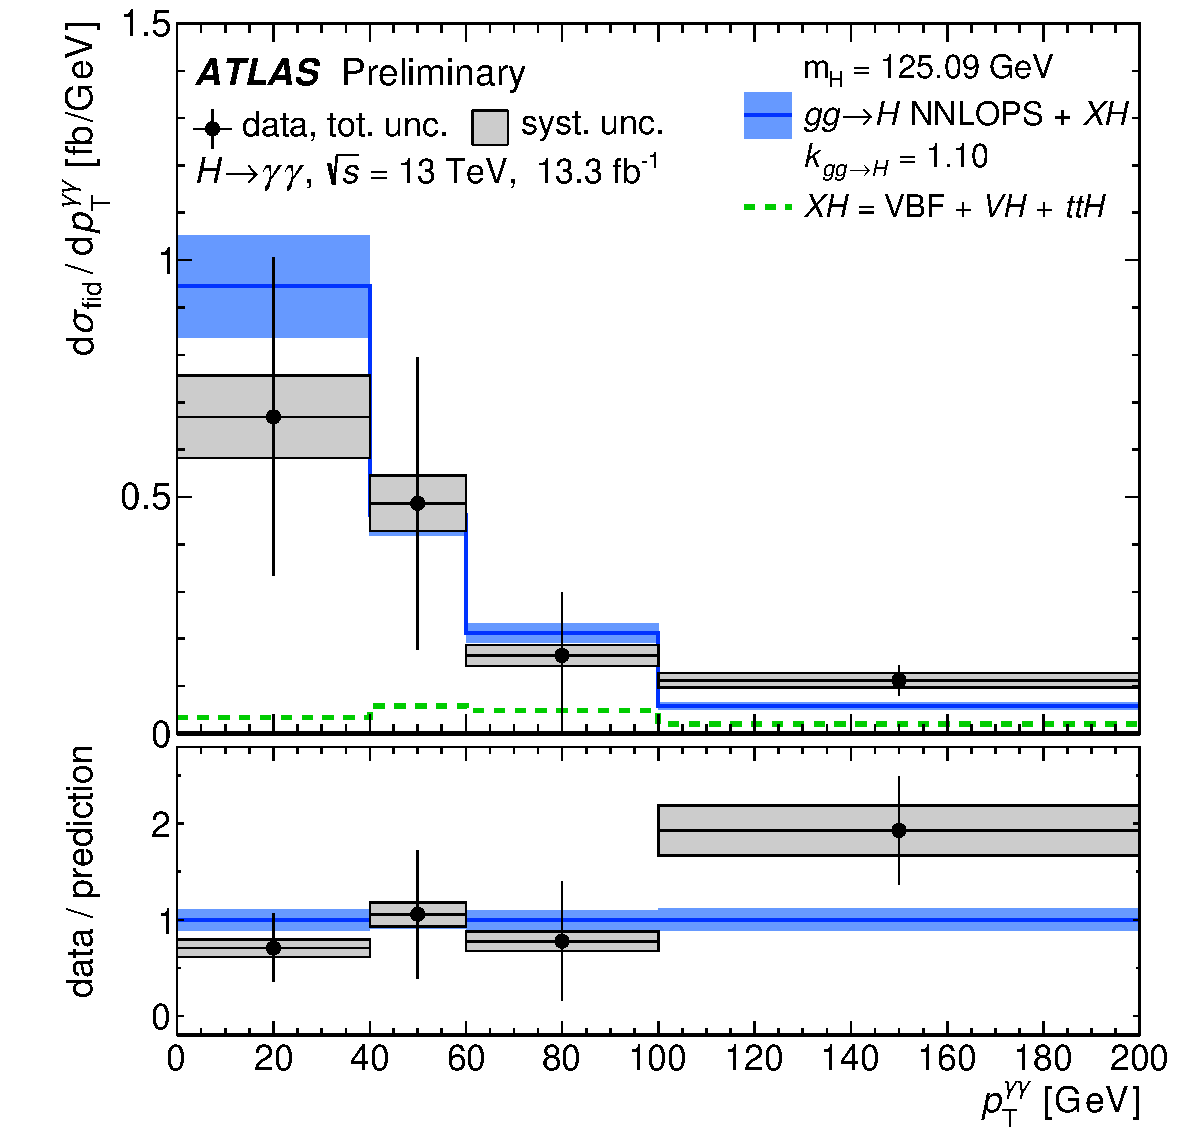
\includegraphics[height=2in]{figures/ATLAS-CONF-2016-067__fig_10a__pTgg.pdf}
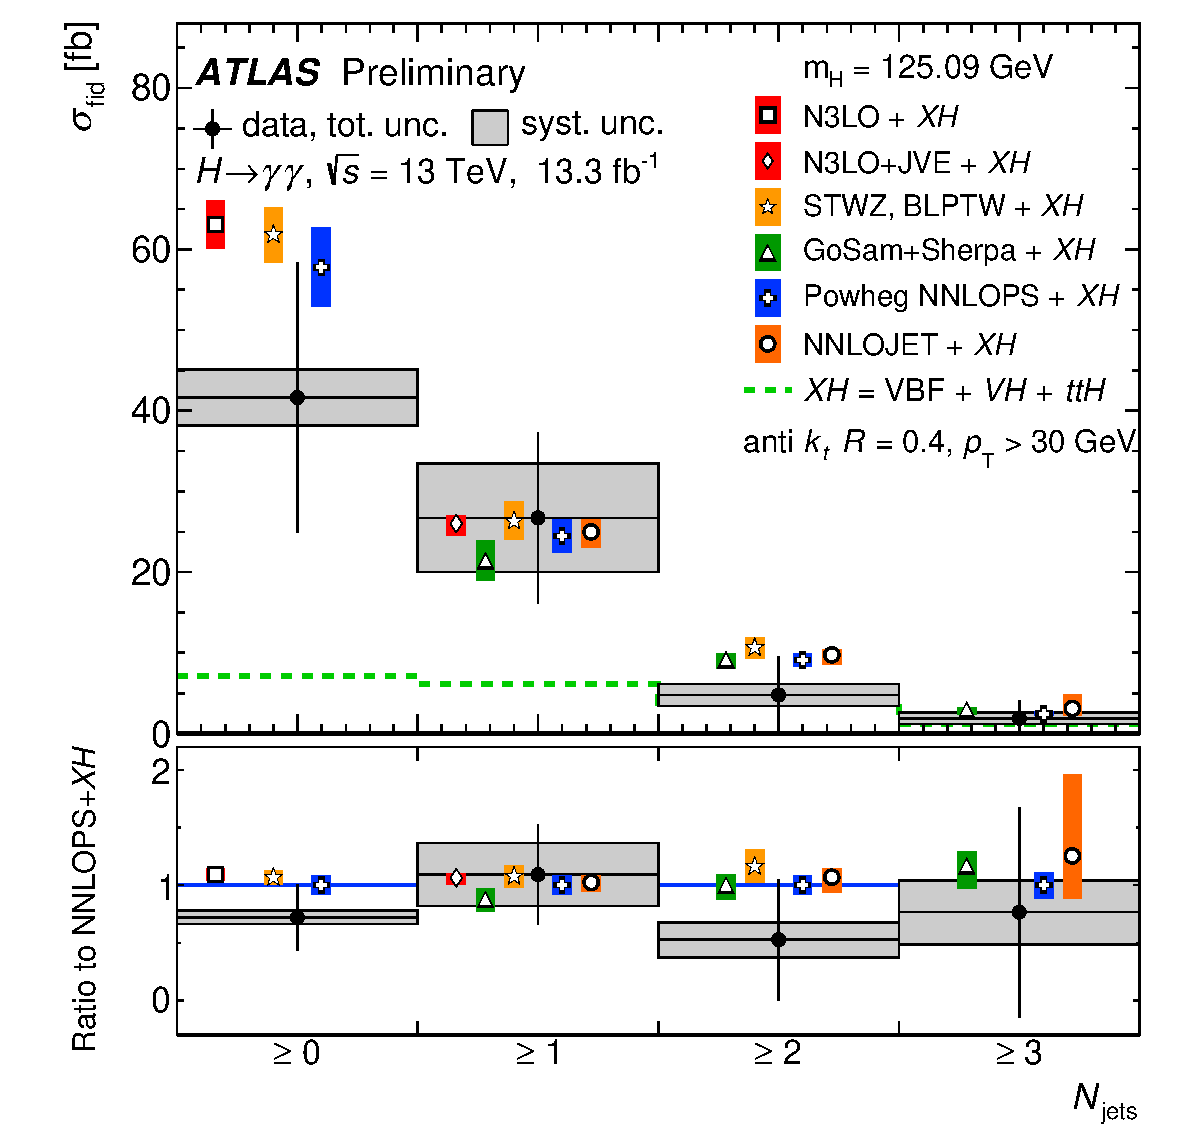
\includegraphics[height=2in]{figures/ATLAS-CONF-2016-067__fig_11b__njets.pdf}\\
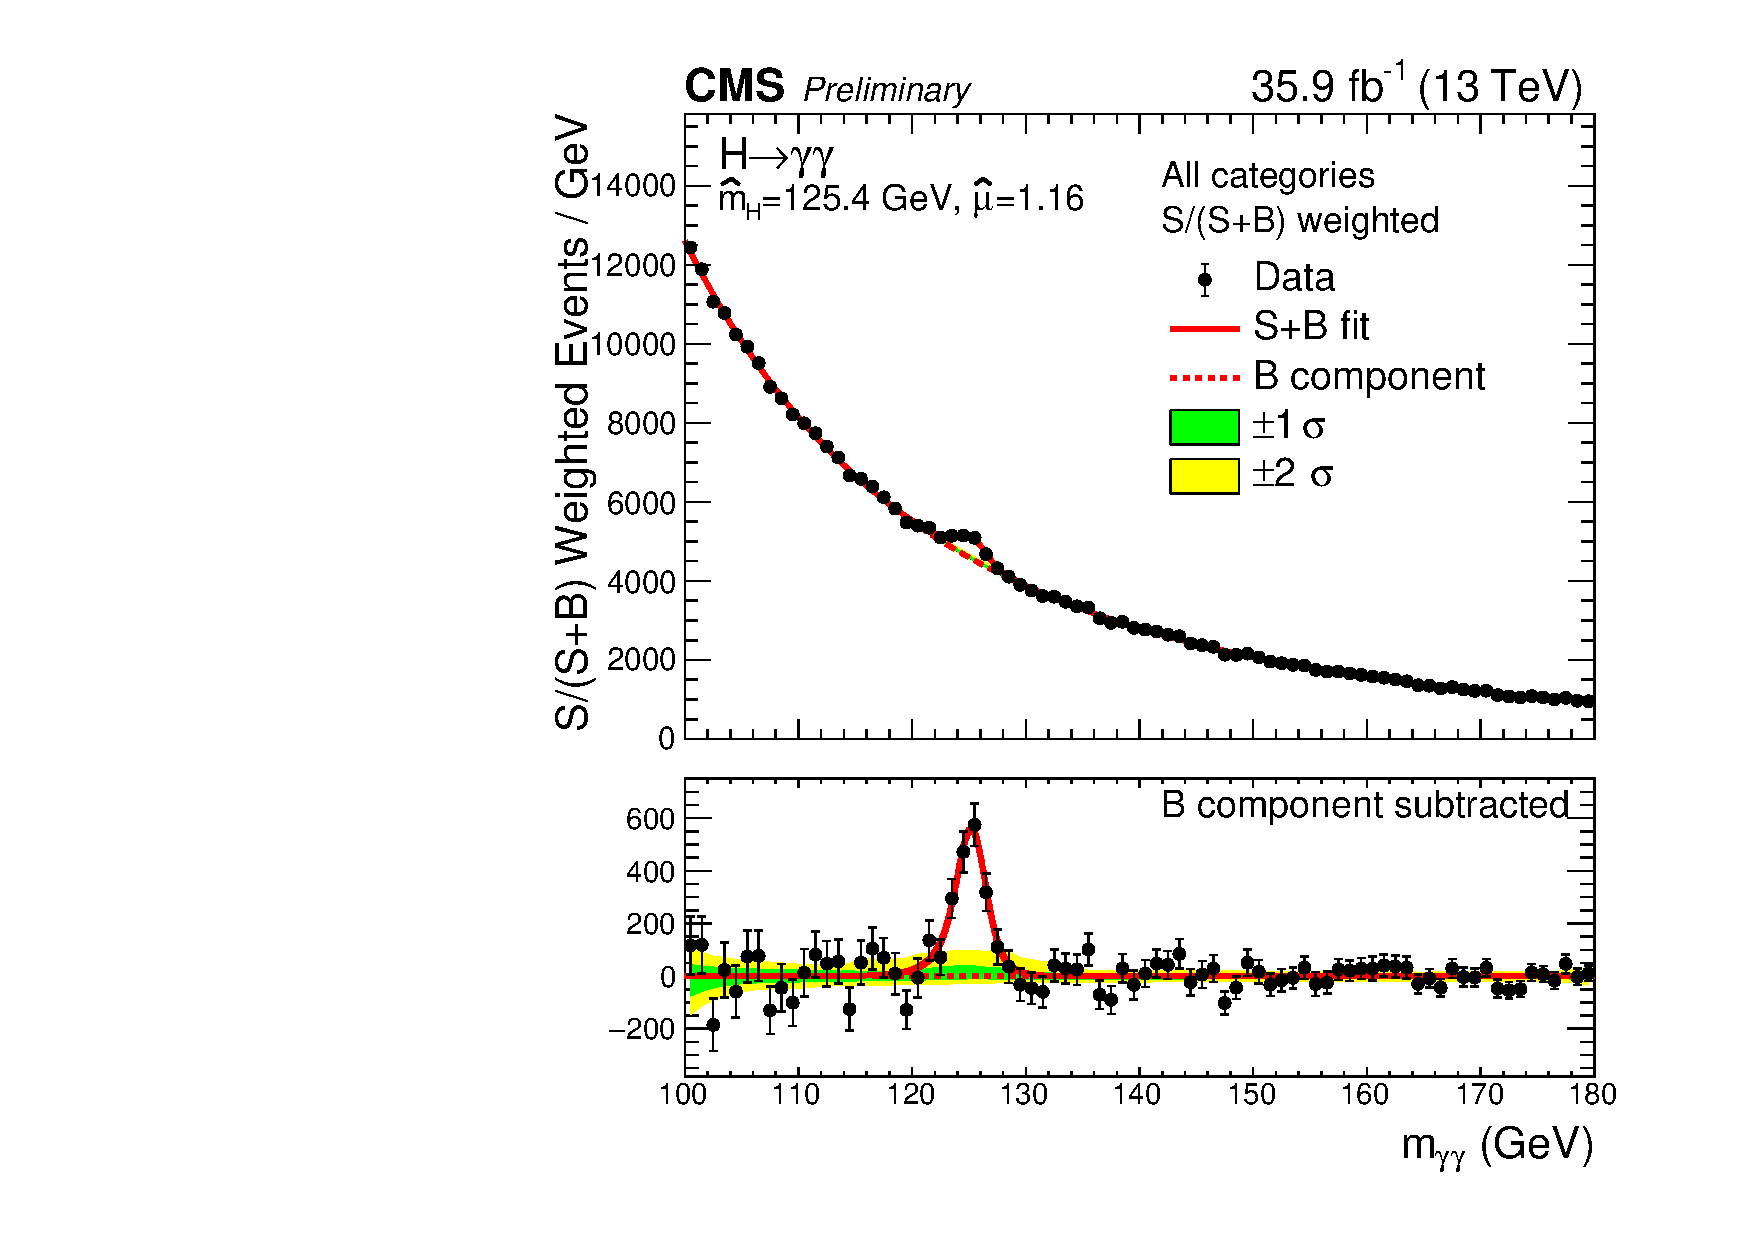
\includegraphics[height=2in]{figures/CMS-HIG-16-040__Figure_013-b__mgg.pdf}
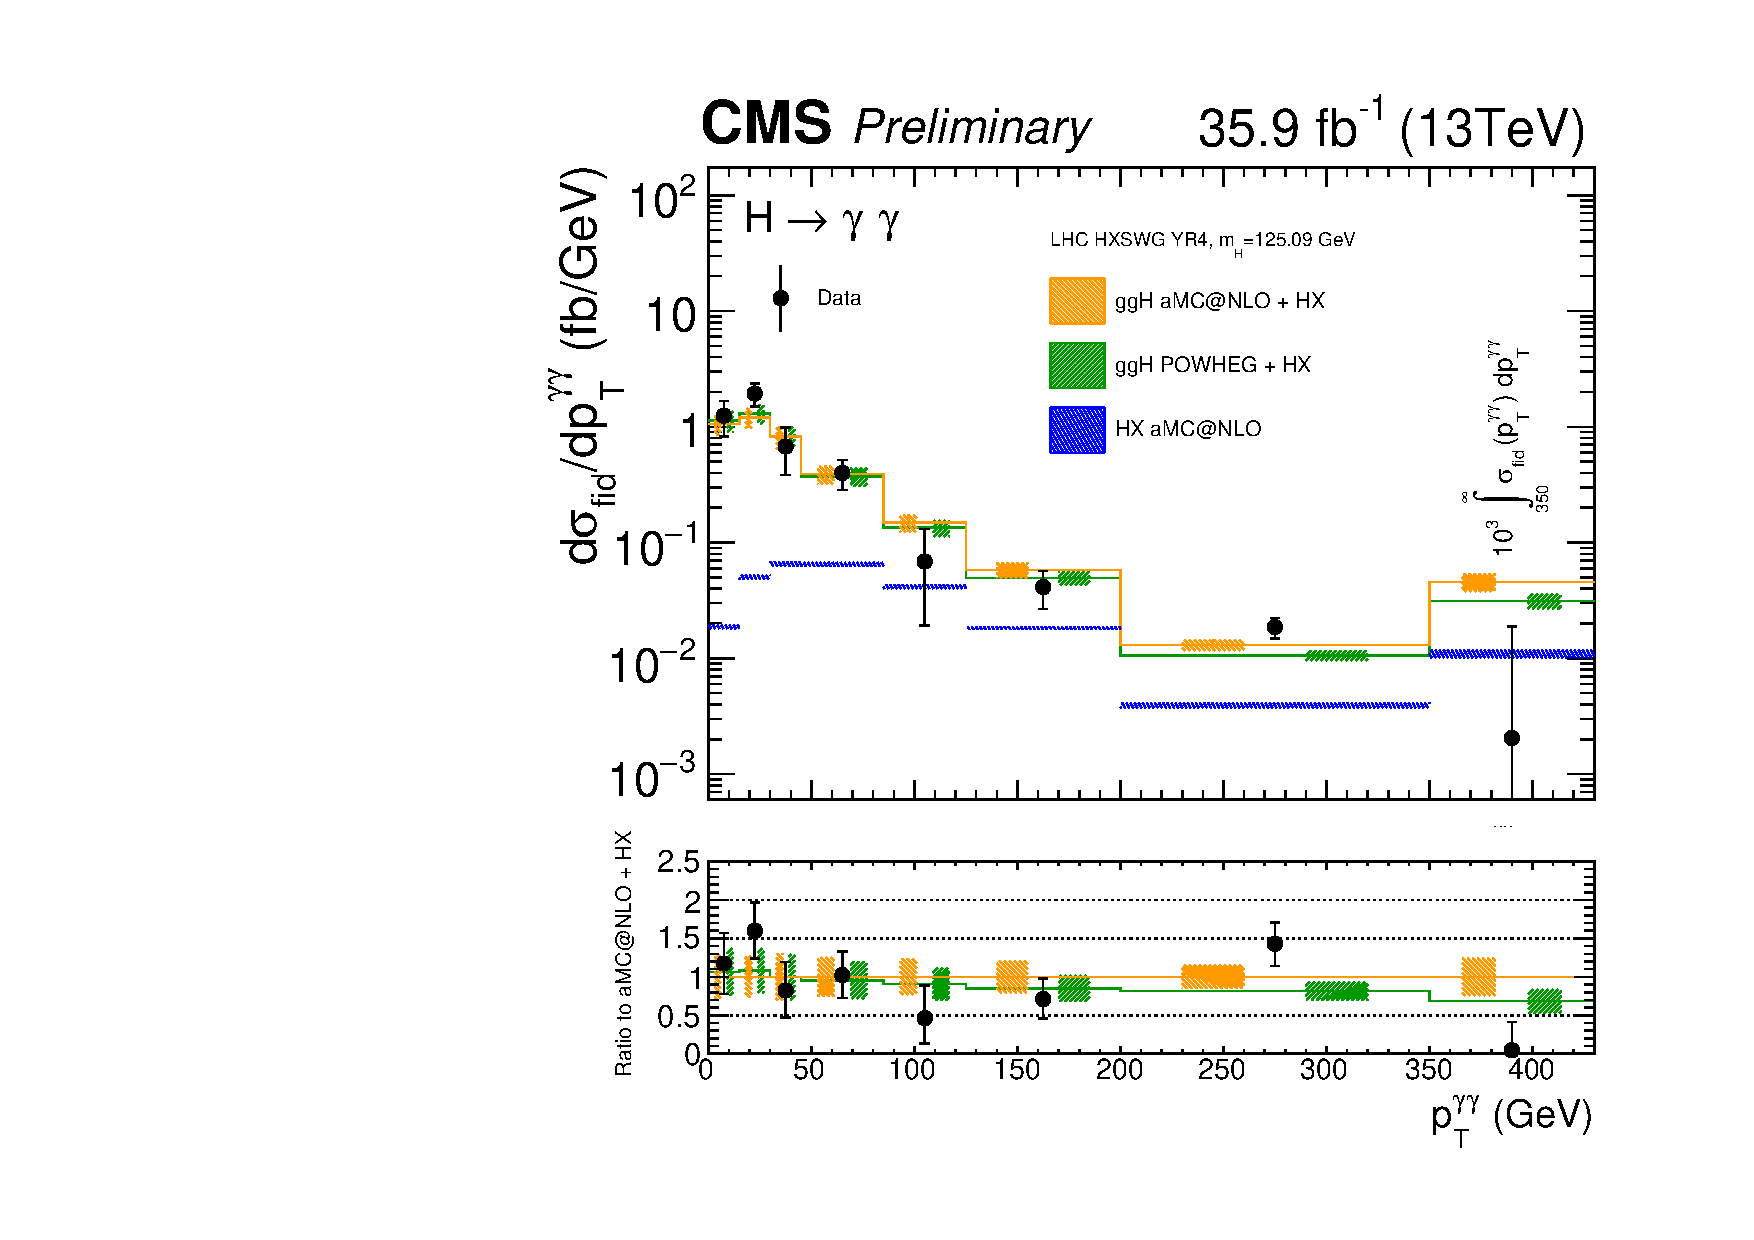
\includegraphics[height=2in]{figures/CMS-HIG-17-015__Figure_004-a__pTgg.pdf}
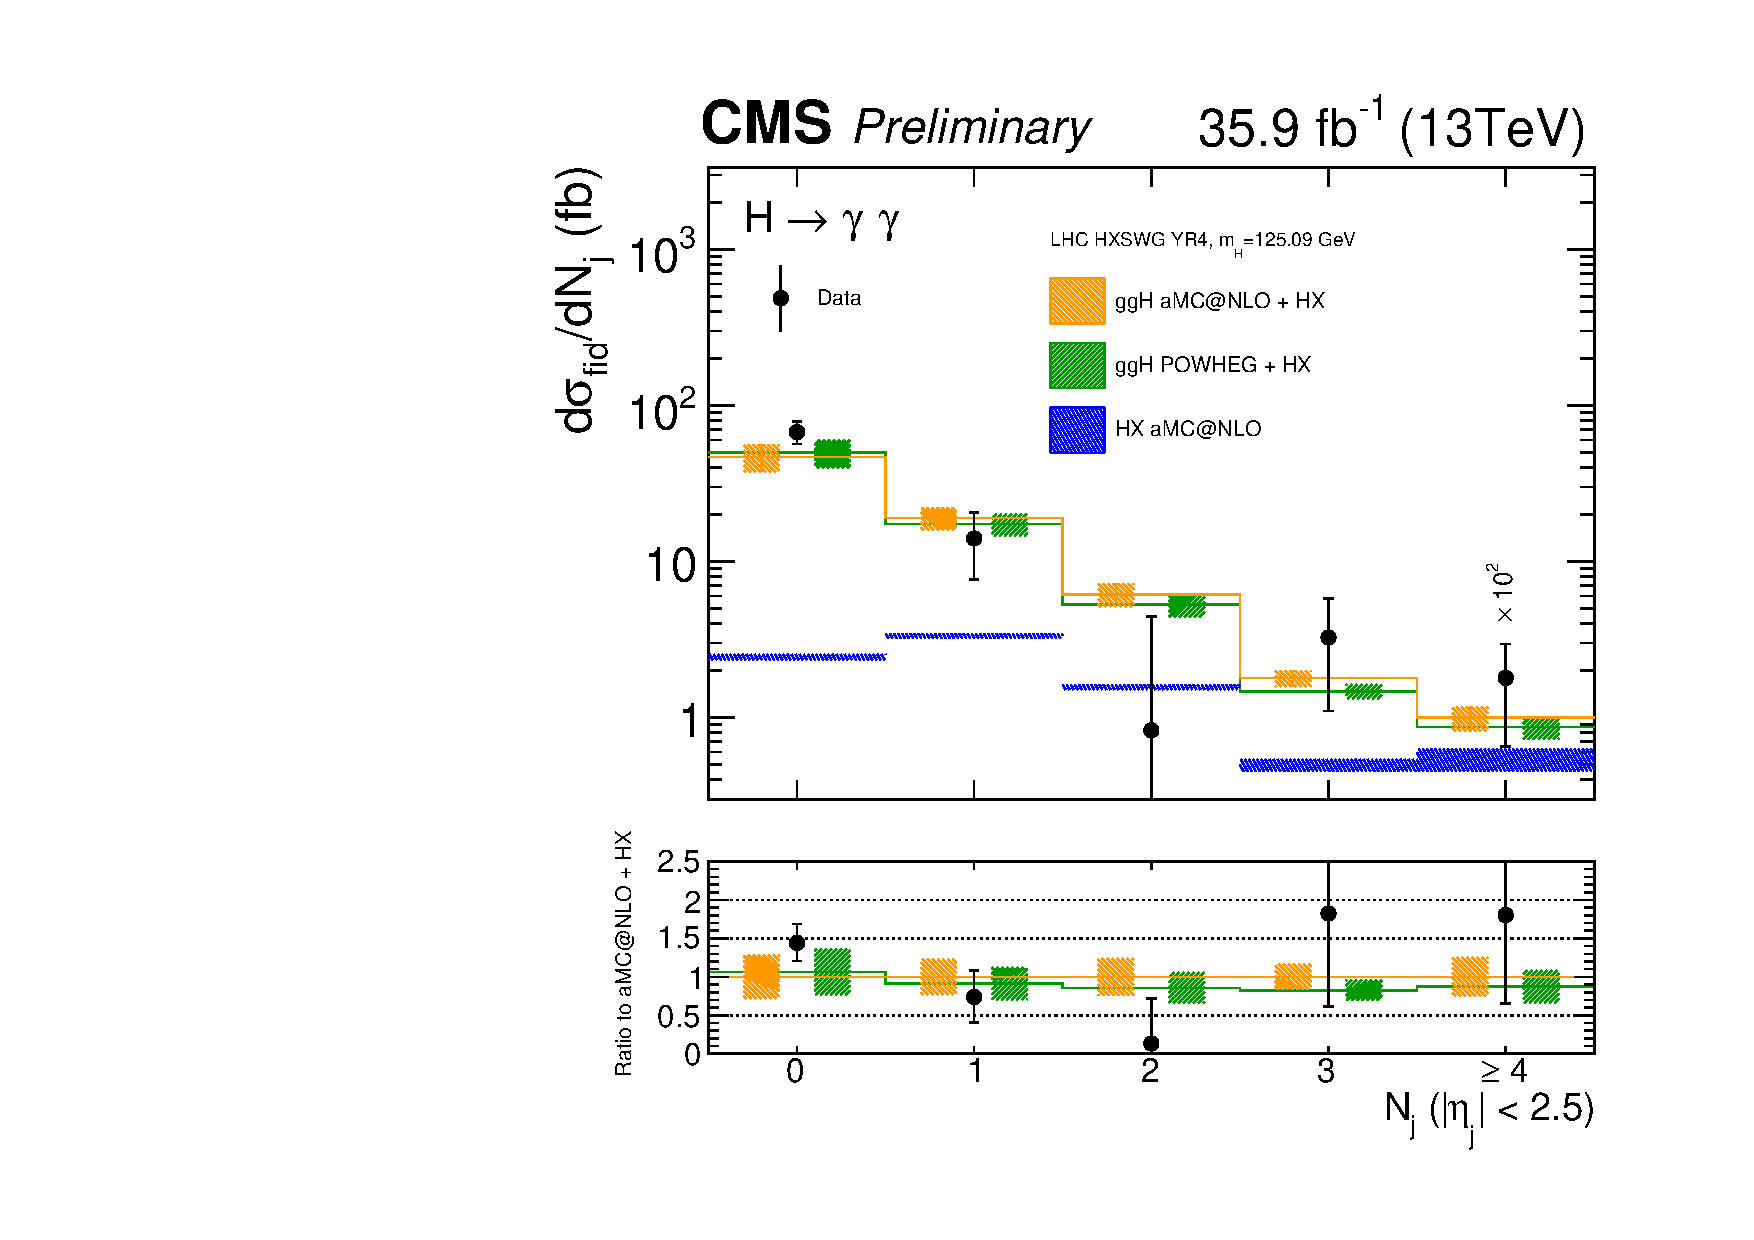
\includegraphics[height=2in]{figures/CMS-HIG-17-015__Figure_004-b__njets.pdf}
\caption{
  (Top left) ATLAS diphoton invariant mass spectrum.
  (Top center and right) ATLAS differential fiducial cross sections, for the
  transverse momentum of the Higgs boson (center) and the number of jets (right).
  (Bottom left) CMS diphoton invariant mass spectrum.
  (Bottom center and right) CMS differential fiducial cross sections, for the
  transverse momentum of the Higgs boson (center) and the number of jets (right).
}
\label{fig:figure-gg}
\end{figure}


%~~~~~~~~~~~~~~~~~~~~~~~~~~~~~~~~~~~~~~~~~~~~~~~~~~~~~~~~~~~~~~~~~~~~~~~~~~~~~~~
\section{\boldmath ${\rm H}\to\tau\tau$}
%~~~~~~~~~~~~~~~~~~~~~~~~~~~~~~~~~~~~~~~~~~~~~~~~~~~~~~~~~~~~~~~~~~~~~~~~~~~~~~~

To establish the mass generation mechanism for fermions, it is necessary to
demonstrate the direct coupling of the scalar boson to fermions, and the
proportionality of its strength to the fermion mass. The most promising decay
channel is $\tau\tau$, because of the large event rate expected in the SM
compared to the other leptonic decay modes, and of the smaller contribution
from background events with respect to the ${\rm b\bar{b}}$ channel. Here we
report the results of a search for the SM scalar boson using $35.9~{\rm fb^{-1}}$
at 13 TeV, when it decays to a pair of $\tau$ leptons~\cite{CMS:2017wyg}. The
four $\tau$-pair final states with the largest branching fractions,
$\mu\tau_{\rm h}$, ${\rm e}\tau_{\rm h}$, $\tau_{\rm h}\tau_{\rm h}$, and
${\rm e}\mu$, are studied.

%%%
%%% TO BE FILLED
%%%

The search for an excess of SM scalar boson events over the expected background
involves a global maximum likelihood fit based on two-dimensional distributions
in all channels, together with control regions for the ${\rm t{\bar t}}$, QCD
multijet and W+jets backgrounds. Figure~\ref{fig:tauhtauh_VBF} shows the
distribution observed, together with the expected background and signal
distributions, in the $\tau_{\rm h}\tau_{\rm h}$ channel and VBF category. The
signal prediction for a scalar boson with $m_{\rm H} = 125$~GeV is
normalized to its best-fit cross section times branching fraction. The background
distributions are adjusted to the results of the global maximum likelihood fit.

\begin{figure}[htb]
\centering
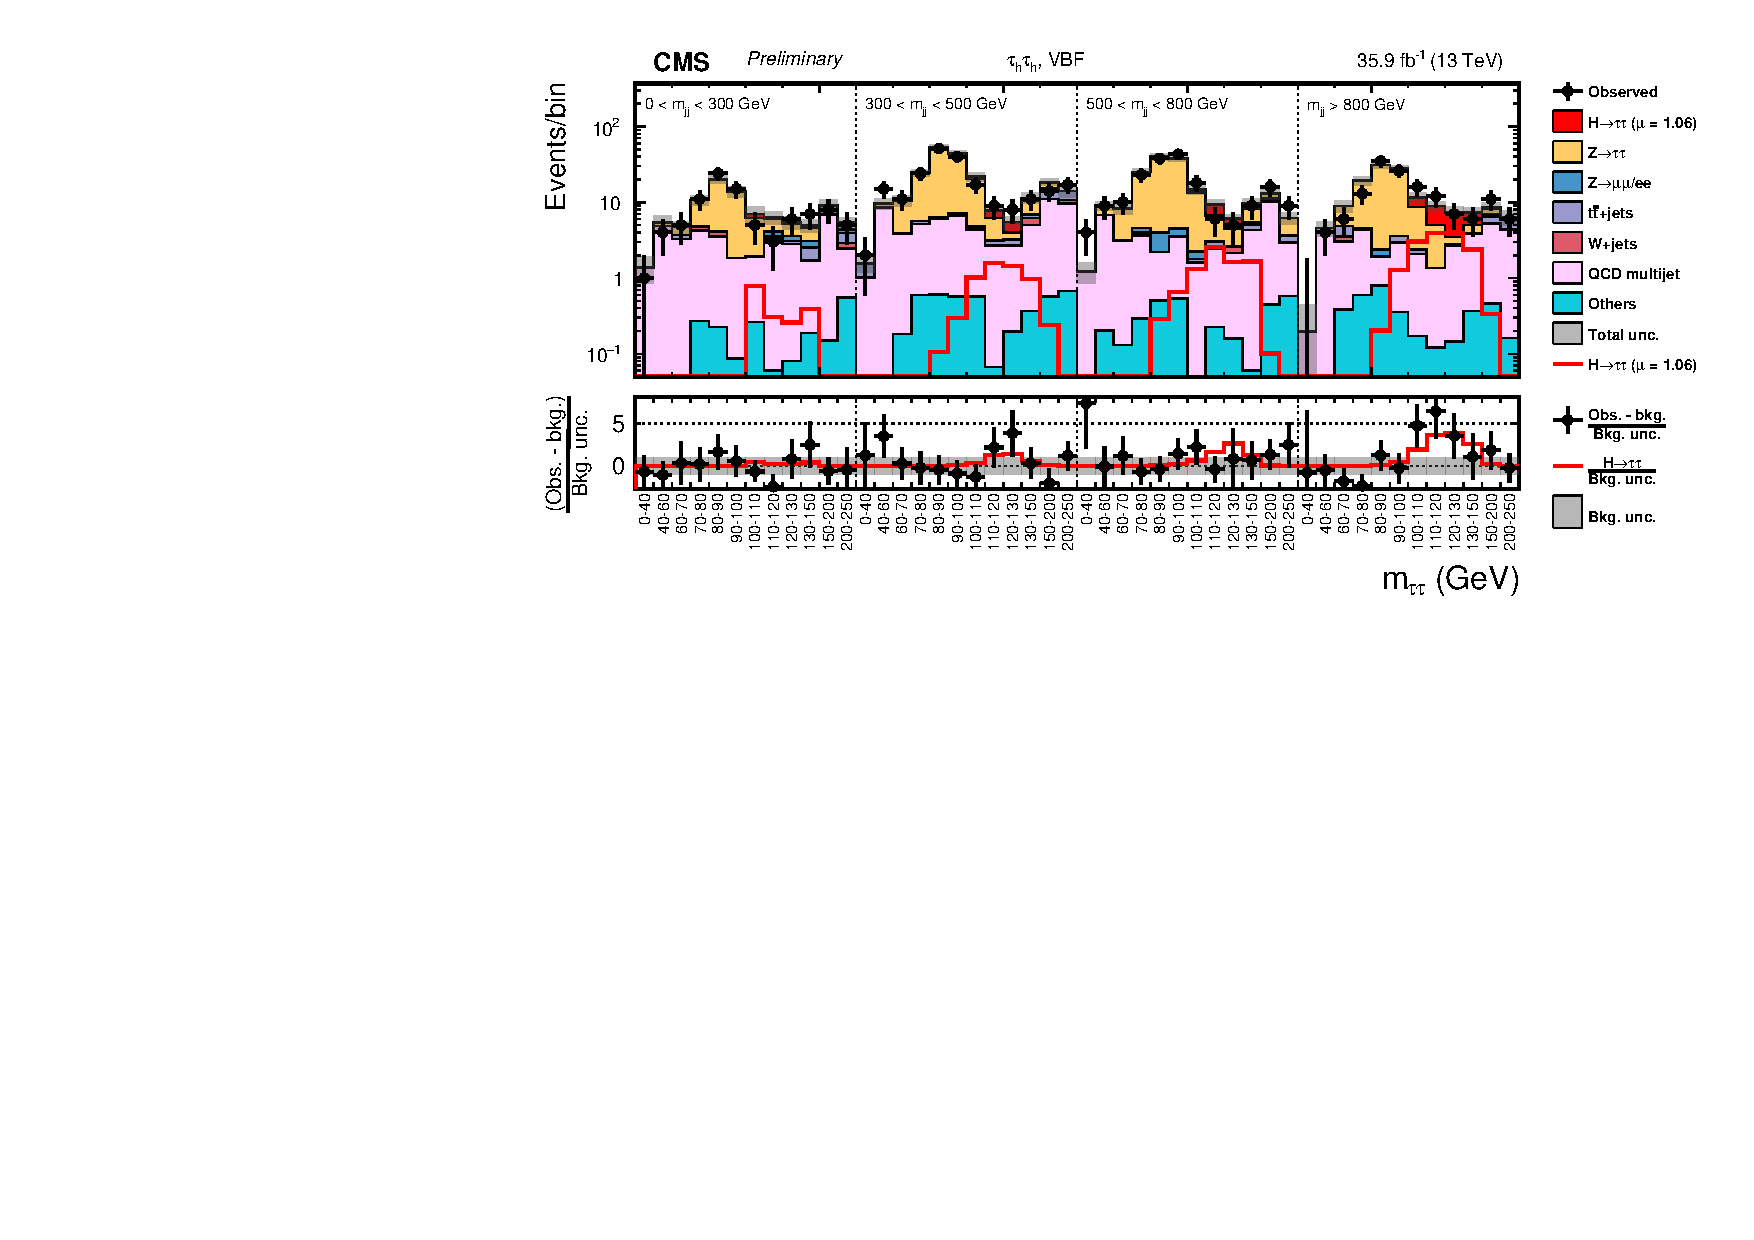
\includegraphics[height=2in]{figures/CMS-HIG-16-043__Figure_013__tauhtauh-VBF.pdf}
\caption{Observed and predicted 2D distributions in the VBF category of the
$\tau_{\rm h}\tau_{\rm h}$ final state. The normalization of the predicted
background distributions corresponds to the result of the global fit. The signal
distribution is normalized to its best-fit signal strength.
}
\label{fig:tauhtauh_VBF}
\end{figure}


%~~~~~~~~~~~~~~~~~~~~~~~~~~~~~~~~~~~~~~~~~~~~~~~~~~~~~~~~~~~~~~~~~~~~~~~~~~~~~~~
\section{Searches for new phenomena}
%~~~~~~~~~~~~~~~~~~~~~~~~~~~~~~~~~~~~~~~~~~~~~~~~~~~~~~~~~~~~~~~~~~~~~~~~~~~~~~~


%~~~~~~~~~~~~~~~~~~~~~~~~~~~~~~~~~~~~~~~~~~~~~~~~~~~~~~~~~~~~~~~~~~~~~~~~~~~~~~~
\section{Conclusions}
%~~~~~~~~~~~~~~~~~~~~~~~~~~~~~~~~~~~~~~~~~~~~~~~~~~~~~~~~~~~~~~~~~~~~~~~~~~~~~~~


%%  if necessary
%% J.Piedra %% \Acknowledgements
%% J.Piedra %% I am grateful to XYZ for fruitful discussions.


\begin{thebibliography}{99}

%%
%%  bibliographic items can be constructed using the LaTeX format in SPIRES:
%%    see    http://www.slac.stanford.edu/spires/hep/latex.html
%%  SPIRES will also supply the CITATION line information; please include it.
%%

\bibitem{Aad:2012tfa} 
  G.~Aad {\it et al.}  [ATLAS Collaboration],
  %``Observation of a new particle in the search for the Standard Model Higgs boson with the ATLAS detector at the LHC,''
  Phys.\ Lett.\ B {\bf 716}, 1 (2012)
  [arXiv:1207.7214 [hep-ex]].
  %%CITATION = ARXIV:1207.7214;%%
  %3009 citations counted in INSPIRE as of 22 Jul 2014
  
  
%\cite{Chatrchyan:2012ufa}
\bibitem{Chatrchyan:2012ufa} 
  S.~Chatrchyan {\it et al.}  [CMS Collaboration],
  %``Observation of a new boson at a mass of 125 GeV with the CMS experiment at the LHC,''
  Phys.\ Lett.\ B {\bf 716}, 30 (2012)
  [arXiv:1207.7235 [hep-ex]].
  %%CITATION = ARXIV:1207.7235;%%
  %2951 citations counted in INSPIRE as of 22 Jul 2014


\bibitem{ATLAS-ZZ}
  G.~Aad {\it et al.}  [ATLAS Collaboration],
  ATLAS-HIGG-2016-25.


%\cite{CMS:2017jkd}
\bibitem{CMS:2017jkd}
  CMS Collaboration [CMS Collaboration],
  %``Measurements of properties of the Higgs boson decaying into four leptons in pp collisions at sqrt{s} = 13 TeV,''
  CMS-PAS-HIG-16-041.
  %%CITATION = CMS-PAS-HIG-16-041;%%
  %4 citations counted in INSPIRE as of 29 May 2017


%\cite{CMS:2017wyg}
\bibitem{CMS:2017wyg}
  CMS Collaboration [CMS Collaboration],
  %``Observation of the SM scalar boson decaying to a pair of $\tau$ leptons with the CMS experiment at the LHC,''
  CMS-PAS-HIG-16-043.
  %%CITATION = CMS-PAS-HIG-16-043;%%


\end{thebibliography}

 
\end{document}
